%!TEX root = ../dokumentation.tex

\chapter{Grundlagen}
\label{cha:Grundlagen}

\section{DocBridge Mill Plus}{
\label{sec:MillPlus}
DocBridge Mill Plus ist eine plattformunabhängige, skalierbare Software für die Anzeige und Verarbeitung von Datenströmen. Sie ermöglicht die Analyse und Modifikation von Dokumenten in verschiedensten Formaten und die Konvertierung in unterschiedliche Ausgangsformate. Die Dokumente lassen sich auf nahezu allen gängigen physikalischen und digitalen Kanälen darstellen. Mit DocBridge Mill Plus ist der Anwender auch in der Lage Prozesse, die im Output-Management üblich sind, abzubilden. Der modulare Aufbau der Software lässt es zu, sie mit zusätzlichen Modulen um Ein-und Ausgabeformate und Workflows zu erweitern.

\begin{figure}[htbp] 
  \centering
     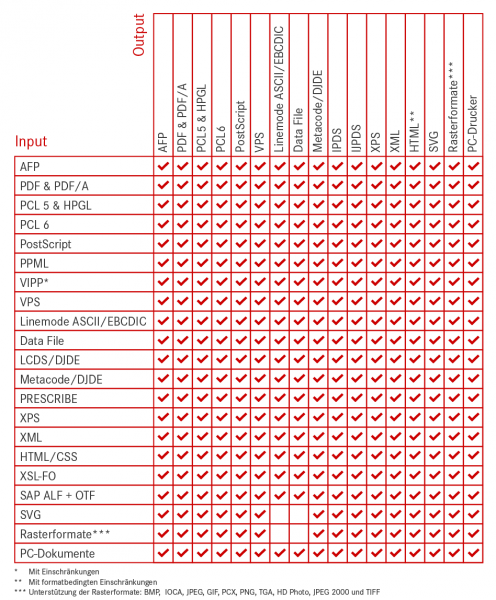
\includegraphics[height=.6\textwidth]{compart_matrix_de.png}
  \caption{Mögliche Verarbeitungsformate der DocBridge Mill Plus}
  \label{fig:compart_matrix}
\end{figure}

\newpage

}

\section{DocBridge Workbench for Mill Plus}{
\label{sec:DBWB}
DocBridge Workbench for Mill Plus bietet eine grafische Benutzeroberfläche für die Filterkonfiguration und die formatunabhängige Dokumentendarstellung. In der \ac{DBWB} können einzelne, mehrere oder in Stapeln zusammengefasste Dokumente angezeigt werden. Es werden alle in Abbildung \ref{fig:compart_matrix} aufgeführten Formate unterstützt. Geladene Dokumente können in der, in Abbildung \ref{fig:dbwb_document} vorgestellten Dokumentenperspektive einheitlich dargestellt werden. Alle Dokumente, die in einem der unterstützten Formaten vorliegen, können im Anzeigebereich untersucht werden. So ist es dem Nutzer möglich, sich unabhängig vom Format des Dokuments, völlig auf dessen Inhalt des zu konzentrieren. In der Prozessperspektive (Abbildung \ref{fig:dbwb_process}) können Verarbeitungsschritte konfiguriert, validiert und lokal ausgeführt werden. Die erstellte Prozesskonfiguration kann exportiert und in der DocBridge Mill Plus ausgeführt werden. Die Konfiguration der Prozesse erfolgt überwiegend über Drag \& Drop. Die Prozessperspektive ist die Standartperspektive der \ac{DBWB}.     

\newpage

\begin{figure}[htbp] 
\centering
     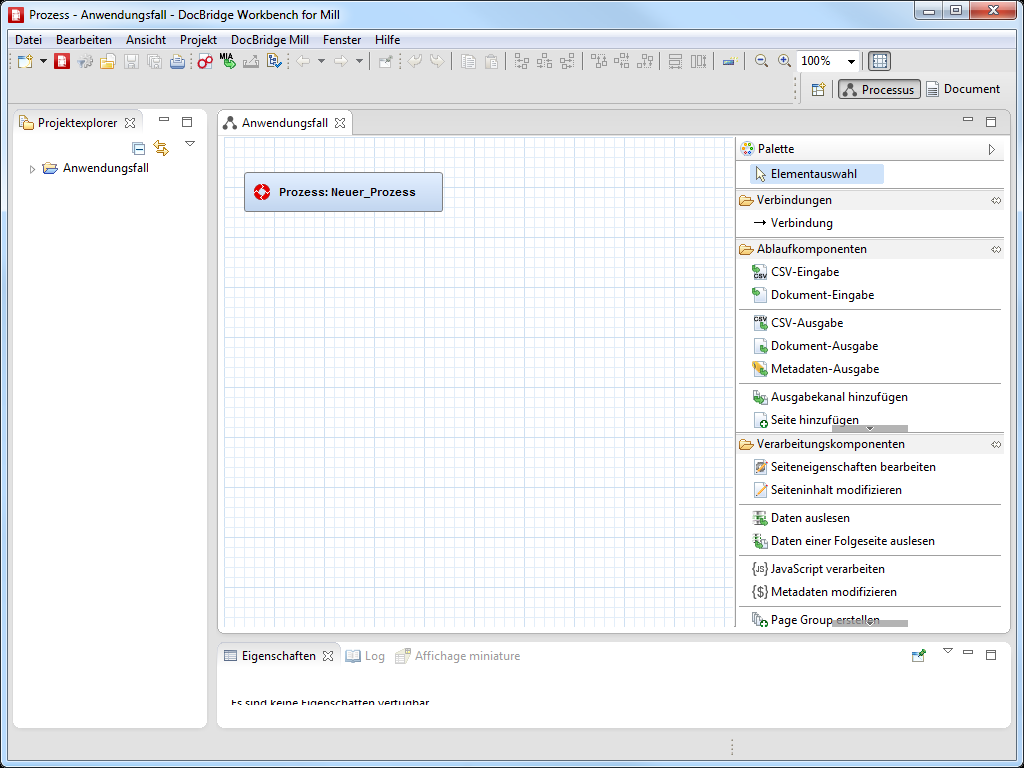
\includegraphics[height=.46\textwidth]{dbwb_process.png}
  \caption{Prozessperspektive}
  \label{fig:dbwb_process}
\end{figure}

\begin{figure}[htbp] 
\centering
     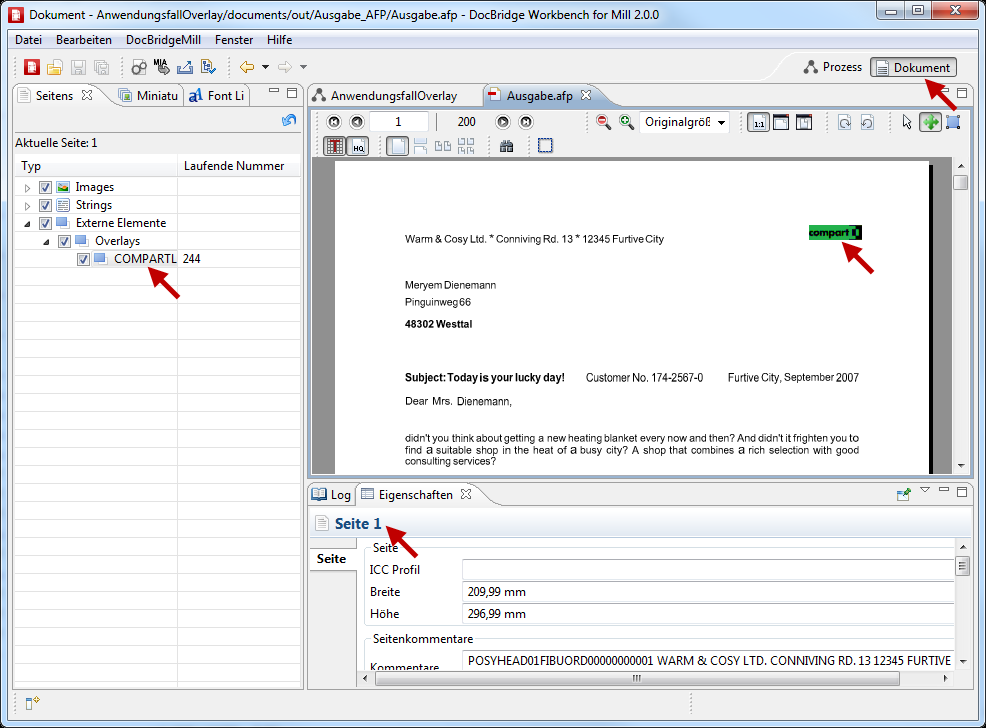
\includegraphics[height=.46\textwidth]{dbwb_document.png}
  \caption{Dokumentperspektive}
  \label{fig:dbwb_document}
\end{figure}


}
\newpage

\section{OSGi}{
\label{sec:OSGi}
\ac{OSGi} Services ermöglichen die Zusammenarbeit einzelner Bundles. Java stellt nur begrenzte Möglichkeiten zur Modularisierung bereit. Java Klassen lassen sich zwar unter der Verwendung von Packages gruppieren, jedoch ist es nicht möglich diese Gruppierungen und Restriktionen zur Laufzeit beizubehalten. Die Möglichkeit, einzelne Klassen als package-protected zu deklarieren ist meist keine befriedigende Lösung. \ac{OSGi} ermöglicht die Verwaltung der Sichtbarkeit von Packages zur Laufzeit. \ac{OSGi} ist ein Framework, welches sich auch dem Problem der Modularisierung annimmt und die Entwicklung von modularen Anwendungen auf der Java-Plattform ermöglicht, was in Abbildung \ref{fig:osgi_layer} veranschaulicht wird. \ac{OSGi}-Anwendungen bestehen aus einzelnen Modulen, die auch Bundles genannt werden. Jedes Bundle hat einen eigenen Lebenszyklus. Dies bedeutet, dass zur Laufzeit einzelne Bundles dynamisch geladen und entfernt werden können. Die Spezifikation von \ac{OSGi} wird von der \ac{OSGi} Alliance erstellt. Die \ac{OSGi} Alliance wurde 1999 von rund 30 namhaften Firmen gegründet, um den Anforderungen im Bereich der eingebetteten Systeme gerecht zu werden. \cite[S.3]{Queue} Die Eclipse \ac{IDE} arbeitet seit Version 3.0 mit der \ac{OSGi} Implementierung Equinox.  

\begin{figure}[htbp] 
\centering
     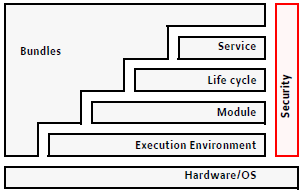
\includegraphics[height=.5\textwidth]{osgi_layer.png}
  \caption{OSGi Schichtenmodell \protect  \cite[aus S.2]{OSGi}}
  \label{fig:osgi_layer}
\end{figure}

}


\section{OSGi Services}{
\label{sec:OSGi_Services}
Bei \ac{OSGi} Services handelt es sich um Java-Objekte, die unter einem Interface in der \ac{OSGi} Service-Registry angemeldet werden. In der Service-Registry angemeldete Services können von anderen Bundles verwendet werden. Services können genau wie OSGi-Bundles dynamisch geladen und entfernt werden. Wird ein Bundle, das einen Service bereitstellt gestoppt, so muss das verwendende Bundle auf das Wegfallen des Service entsprechend reagieren. \cite[vgl.S.114]{OSGi}
}

\section{SWT}{
\label{sec:SWT}
Das \ac{SWT}  stellt das Framework für grafische Oberflächen auf der Eclipse-Plattform bereit. \ac{SWT} stellt eine Java Schnittstelle für die nativen GUI-Bibliotheken verschiedener Betriebssysteme zur Verfügung. Hierzu gehören Microsoft Windows, Linux\footnote{GIMP Toolkit} und Mac OS X\footnote{Cocoa}. Da auf die spezifischen Steuerelemente des jeweiligen Betriebssystems zugegriffen wird, kann mit SWT auf den oben genannten Plattformen ein natives Aussehen und Verhalten erzielt werden, wie in Abbildung \ref{fig:swt_plattform} veranschaulicht wird.


\begin{figure}[htbp] 
  \centering
     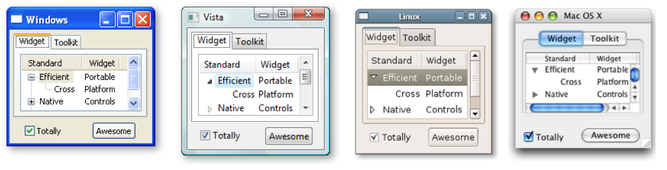
\includegraphics[height=.25\textwidth]{swt_plattform.png}
  \caption{Darstellung von SWT-Widgets auf verschiedenen Betriebssystemen\footnotemark}
   \label{fig:swt_plattform}
\end{figure}
\footnotetext{aus \cite{RalfEbert}}




}

\section{Eclipse RCP}{
\label{sec:Eclipse_rcp}
Eclipse \ac{RCP} ist eine Plattform zur Entwicklung von Desktop-Anwendungen. Sie entstand aus der Eclipse \ac{IDE}, die sich aufgrund ihrer allgemeinen Natur anbietet. Das Eclipse \ac{RCP} Grundgerüst kann durch eigene Anwendungsfunktionalitäten erweitert werden. Viele der vorhandenen Komponenten können in eigenen Anwendungen im Workbench- Aufbau genutzt werden. Als Beispiel wären hier Komponenten für eine Hilfe-Funktion oder das erweiterbare Plug-in-System zu nennen. Vorteile der Anwendungsentwicklung mit Hilfe von Eclipse \ac{RCP} sind Grundstrukturen für den Aufbau von GUI-Anwendungen und der modulare Aufbau. Dieser ermöglicht es, dass Erweiterungen auf Eclipse \ac{RCP} Basis miteinander harmonieren. Die zum implementieren benötigten Werkzeuge sind bereits in der Eclipse \ac{IDE} (Eclipse for RCP/Plug-in Developers)bereits enthalten.
}

\section{Target Platform}{
Eclipse \ac{RCP} Applikationen werden für eine konfigurierbare Zielplattform\footnote{Target Platform} entwickelt. Alle externen Abhängigkeiten werden über die Target Platform geladen. Soll mit Plug-ins die Eclipse \ac{IDE} selbst erweitert werden, verwendet man die standardmäßig die Eclipse \ac{IDE} selbst als Target Platform. \cite[vgl.S14]{RalfEbert} Bei der Entwicklung einer eigenen Rich Client Platform, oder Plug-ins für eine solche, ist es nötig eine eigene Target Platform zu nutzen, da sonst alle Plug-ins und Funktionalitäten der Standard Eclipse IDE auch in der eigenen Applikation wiederzufinden wären. Durch die Definition der Target Platform kann festgelegt werden, in welcher Version der Applikation bestimmte Plug-ins eingebunden werden. Im Idealfall arbeiten alle Entwickler eines Projekts mit der selben Target Platform. So wird eine einheitliche Entwicklungsumgebung sichergestellt.
}

\section{Plug-in zur Profilkonvertierung}{
Vom Studierenden wurde während der letzten Praxiseinheit ein Plug-in im \ac{OSGi}-Umfeld entwickelt, welches dazu verwendet werden kann Filterprofile zu aktualisieren. Die Konfiguration von Konvertierungsabläufen wird in Filterprofilen festgehalten. Deren Aufbau ist in einem XML-Schema definiert. Kommen Funtionalitäten oder Komponenten hinzu, wird das Schema aktualisiert und somit abgeändert. Bestehende Filterprofile sind nun nicht mehr zum Schema valide. Das Plug-in zur Profilkonvertierung liest die Informationen aus dem alten Profil mit Hilfe von verschiedenen Java \ac{API}s aus und generiert anhand des Schemas ein neues Profil, das zum Schema valide ist. Es kommen vor allem die \ac{API}s  Jsoup\footnote{API zum Arbeiten mit degeneriertem HTML} und JaxB\footnote{API für das Erstellen von Klassen aus einer XML-Schema-Instanz} zur Verwendung.
}

